\subsection{K-means}

En la figura \ref{fig:kmeans} se muestran las tablas de confusión resultantes de aplicar el algoritmo de K-means descrito en la sección \ref{sec:kmeans} usando el inicializador k-means++ y uno aleatorio.

\begin{figure}[H]
    \centering
    \begin{subfigure}{8.4cm}
        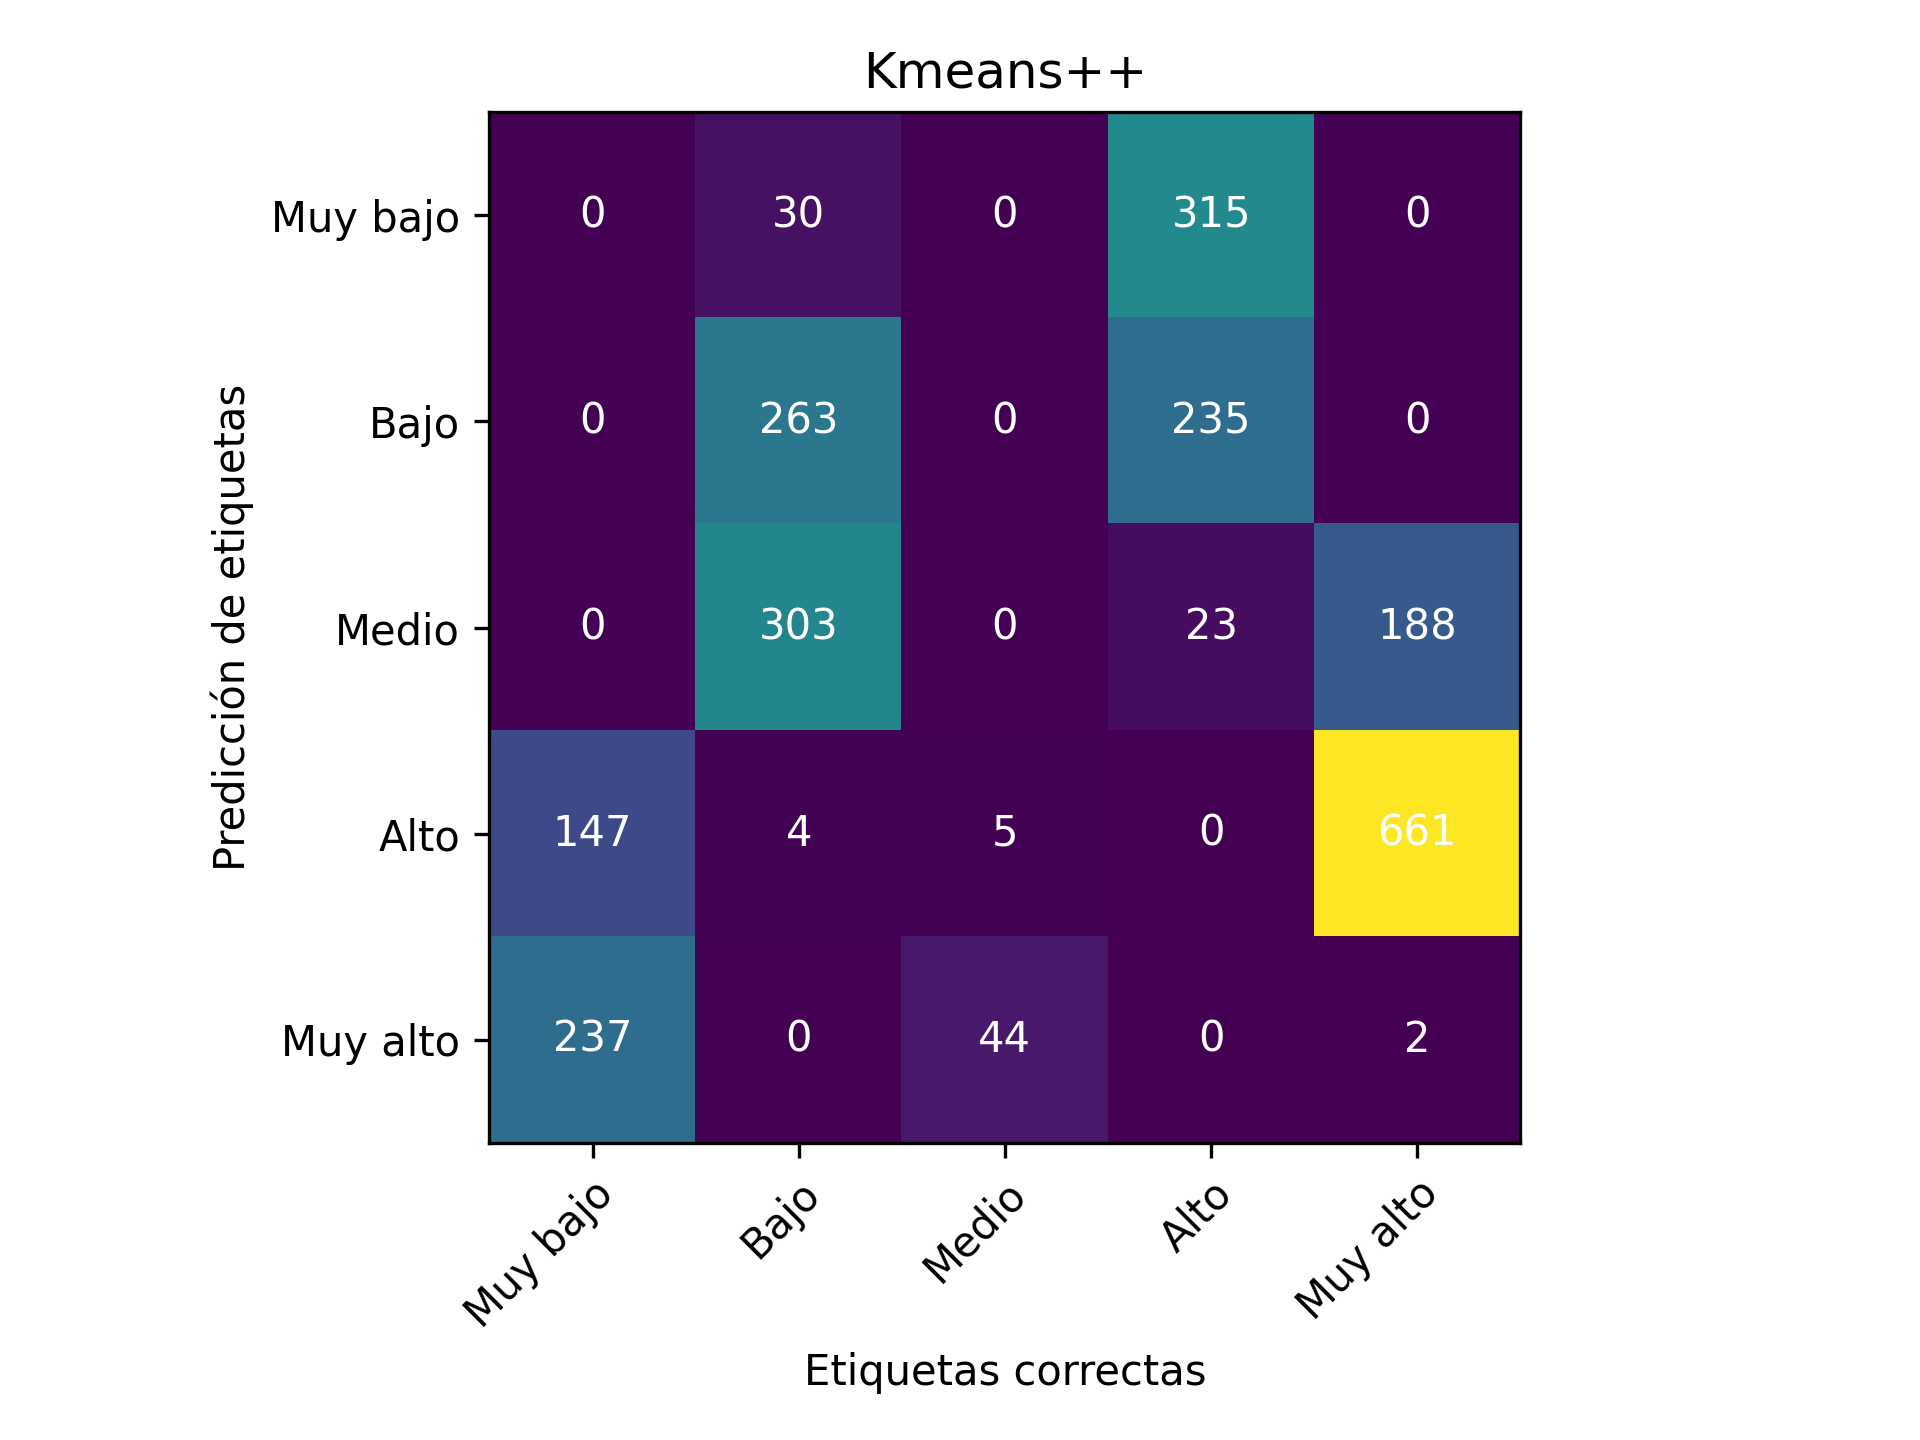
\includegraphics[width=1\linewidth]{Graphics/Data_2015/Kmeans++_confusion_matrix.png}
        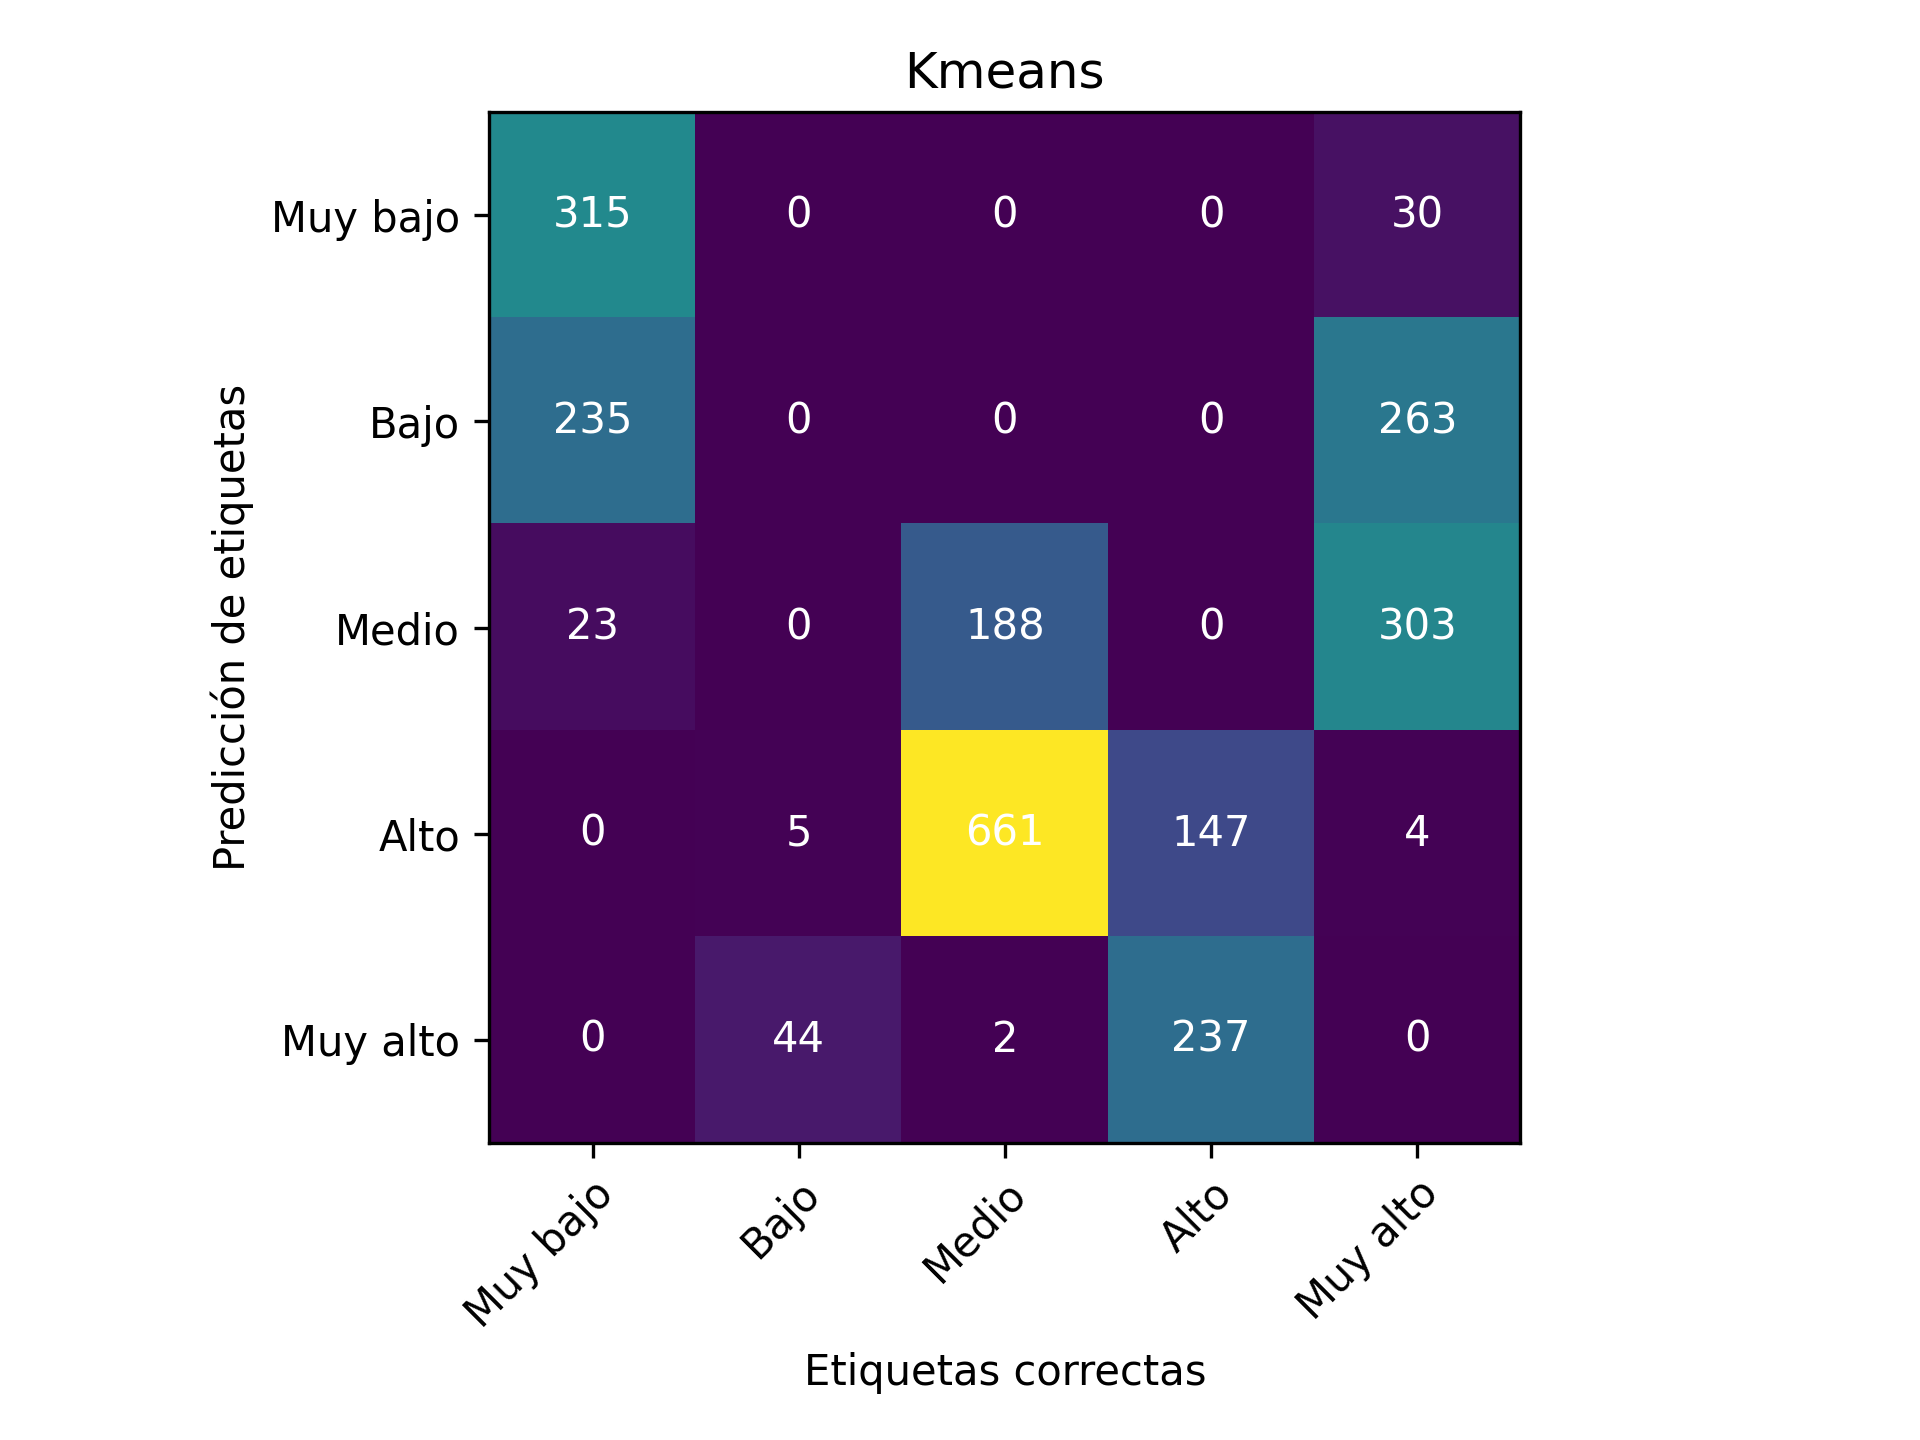
\includegraphics[width=1\linewidth]{Graphics/Data_2015/Kmeans_random_confusion_matrix.png}
        \caption{Datos 2015}
    \end{subfigure}
    \begin{subfigure}{8.4cm}
        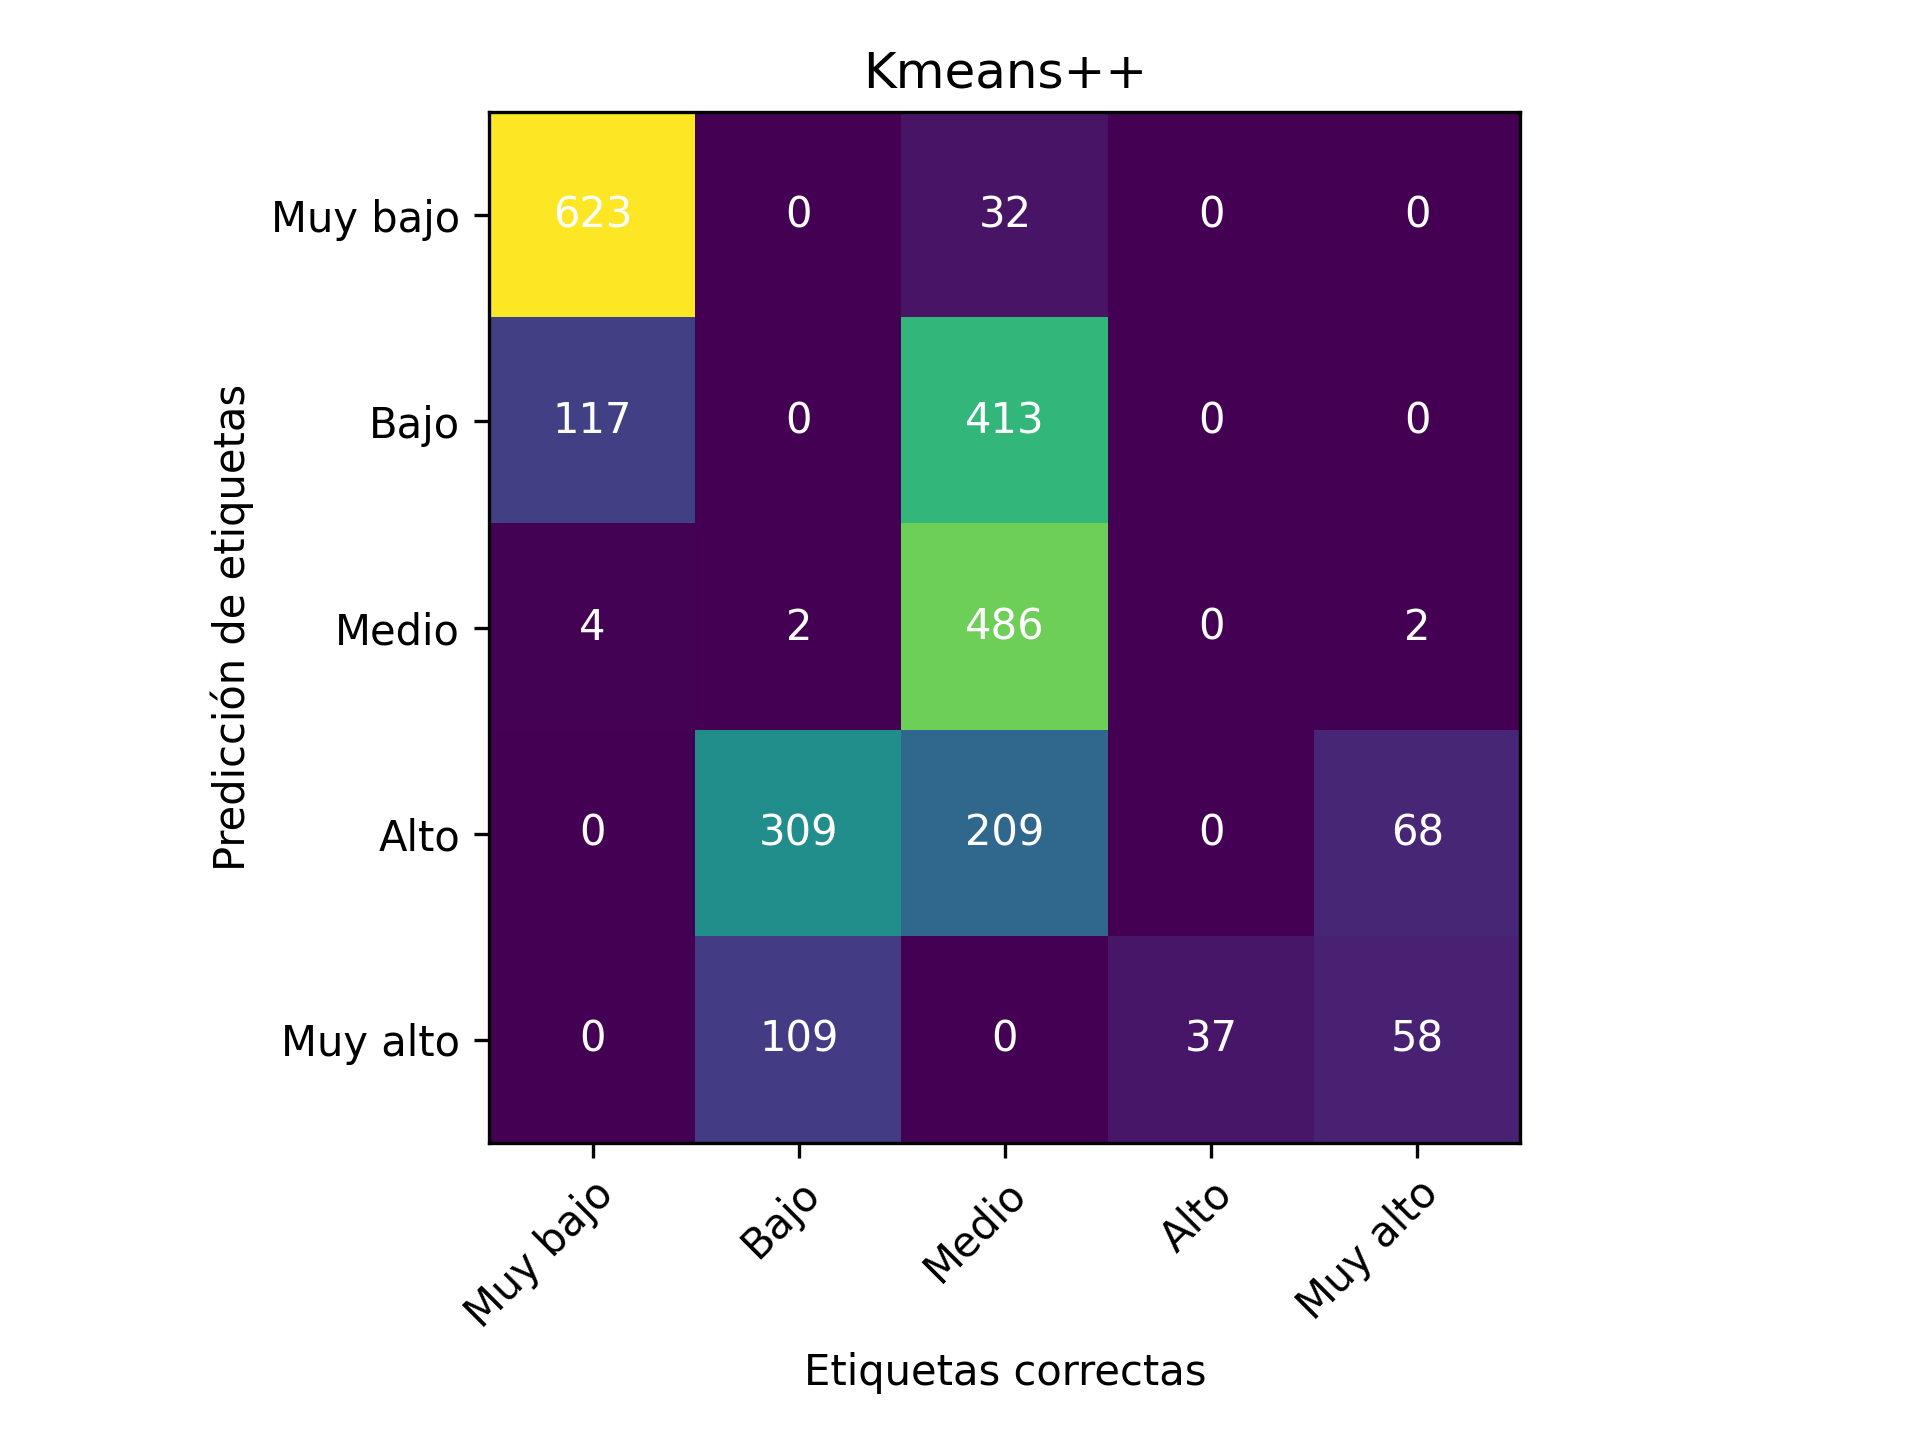
\includegraphics[width=1\linewidth]{Graphics/Data_2020/Kmeans++_confusion_matrix.png}
        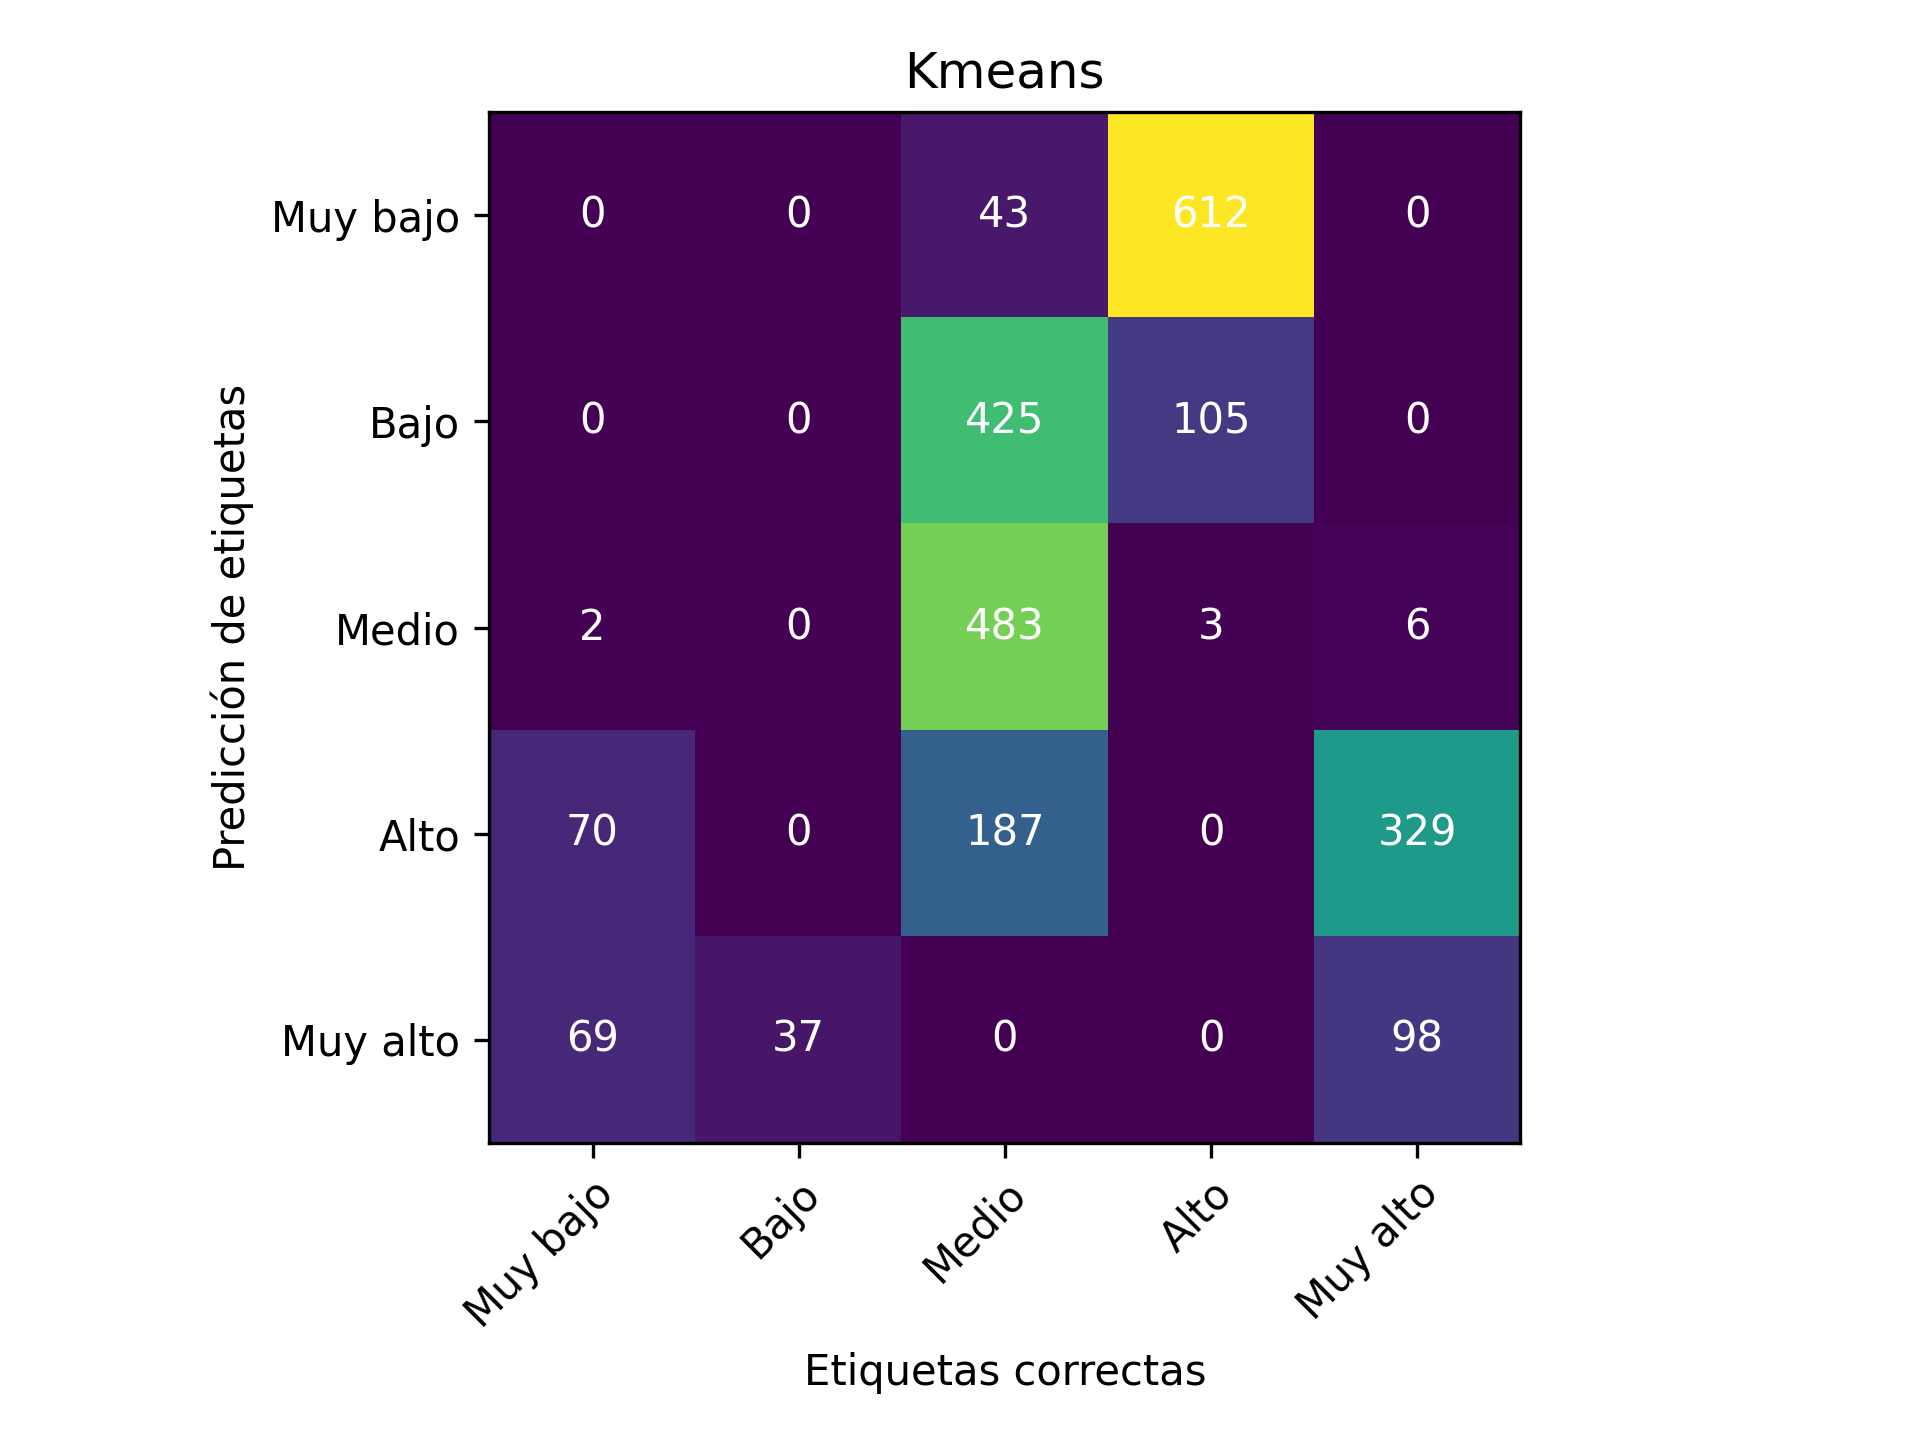
\includegraphics[width=1\linewidth]{Graphics/Data_2020/Kmeans_random_confusion_matrix.png}
        \caption{Datos 2020}
    \end{subfigure}
    \caption{Resultados de aplicar K-means para los datos de índice de marginación de los años 2015 y 2020.}
    \label{fig:kmeans}
\end{figure}